\documentclass[conference]{IEEEtran}
\IEEEoverridecommandlockouts

% IEEEtran selects Times (ptm). Missing PSNFSS metrics (ptmr7t.tfm) causes
% "Font ... ptmr7t ... not loadable". Install texlive-fonts-recommended for Times;
% otherwise Latin Modern (usually in base TeX) is loaded here.
\IfFileExists{ptmr7t.tfm}{}{%
  \typeout{** Times (ptmr7t.tfm) not found: loading Latin Modern. Install texlive-fonts-recommended for IEEE Times.}%
  \usepackage{lmodern}%
}

% Omit \usepackage{cite} so minimal TeX installs without cite.sty still build.
% For IEEE-style citation sorting/compression, install the `cite` package (e.g.
% texlive-latex-recommended on Debian/Ubuntu) and uncomment the next line.
% \usepackage{cite}
\usepackage{amsmath,amssymb,amsfonts}
\usepackage{graphicx}
\usepackage{textcomp}
\usepackage{url}

% --- Metadata placeholders: replace before submission ---
\newcommand{\PaperTitle}{Vanguard Directions in Deep Learning Models: A Survey Research}
% Uncomment and edit if funding applies:
% \newcommand{\PaperFundingThanks}{This work was supported by ...}

\begin{document}

\title{\PaperTitle\\
}

\author{\IEEEauthorblockN{Alejandro Castro López}
\IEEEauthorblockA{\textit{MNA} \\
\textit{ITESM}\\
a00806170@tec.mx}
\and
\IEEEauthorblockN{Arnulfo Alejandro Cavazos Villarreal}
\IEEEauthorblockA{\textit{MNA} \\
\textit{ITESM}\\
a01796489@tec.mx}
\and
\IEEEauthorblockN{Edmundo Carmona Galindo}
\IEEEauthorblockA{\textit{MNA} \\
\textit{ITESM}\\
a01796647@tec.mx}
\and
\IEEEauthorblockN{Luis Daniel Castillo Alegria}
\IEEEauthorblockA{\textit{MNA} \\
\textit{ITESM}\\
a01224696@tec.mx}
}

\maketitle

\begin{abstract}
This survey paper synthesizes a set of recent studies at the leading edge of artificial intelligence research. The topics range widely---from extreme depth in reinforcement learning and reasoning-centric large language model methods, to inference-time scaling, memory efficiency, evaluation of model diversity and homogeneity, reliability of multi-agent systems, and human-centered robot learning. We argue that these works, taken as a group, expose complementary pressures: the push toward more capable systems on one side, and the growing need to understand their limitations, deployment costs, and interaction with users on the other. Rather than attempting exhaustive coverage of each field, we organize the discussion around thematic groupings and foreground what we see as the most pressing open questions about scaling, reliability, and responsible use as models and agents become more pervasive.
\end{abstract}

\begin{IEEEkeywords}
Deep learning, large language models, reinforcement learning, reasoning, inference efficiency, multi-agent systems, human feedback, survey.
\end{IEEEkeywords}

\section{Introduction}
AI models are now embedded in an extraordinary range of applications, from consumer-facing tools to the internal workflows of researchers and developers. Understanding where the field stands---and where it is heading---matters more than ever.
\newline
This survey offers a compact overview of recent deep learning research. The sources we cover span a broad set of concerns: scaling depth in reinforcement learning, reasoning and diversity in language models, inference-time efficiency, failure analysis in multi-agent systems, and lightweight human feedback for robotics. We do not claim comprehensive coverage. Instead, we have selected works that, in our view, illuminate productive tensions the field must navigate as systems grow more capable and more widely deployed.

\section{Background and terminology}

\paragraph{Attention sinks} Attention sinks are a known failure mode of attention mechanisms in which the attention mechanism becomes saturated and the model becomes unable to attend to new information. This is a problem because it can cause the model to hallucinate or produce incorrect answers.

\paragraph{Chain-of-thought (CoT)} Modern surveys of reasoning-centric language models distinguish \emph{chain-of-thought} (CoT) prompting and training from \emph{reinforced} or preference-tuned variants that treat multi-step reasoning as a policy-learning problem \cite{xu2025reasoning}. Related work also studies \emph{recursive} or dynamically structured CoT, where the model allocates extra reasoning depth where needed rather than using a fixed template \cite{sinha2025drcot}.

\paragraph{Inference-time compute} Across this paper, \emph{inference-time compute} refers to additional forward passes, sampling, or search at deployment, as opposed to parameters updated during training; the \emph{key--value (KV) cache} stores attention states so long contexts and long generations do not recompute full attention from scratch each step.

\paragraph{Preference-based learning} \emph{Preference-based learning} denotes training from ranked options, corrections, or light human signals rather than dense demonstrations.

\paragraph{Multi-agent systems (MAS)} A \emph{multi-agent system} composes two or more LLM-based agents that interact---through message passing, shared memory, or orchestrated workflows---to solve tasks that exceed the scope of a single model call.

\section{Scaling depth and reinforcement learning}
How deep is deep enough? Wang \emph{et al.}\ tackle this question in a self-supervised reinforcement learning setting, and the answer turns out to be surprising \cite{wang2025thousand}. They report that increasing depth can unlock goal-reaching behaviors that shallower stacks simply do not exhibit---not just marginally better sample efficiency or reward, but qualitatively different capabilities. This is an important distinction. It suggests that depth is not merely a knob for incremental accuracy; at certain thresholds, it enables the agent to represent or plan in ways that were previously inaccessible.

Figure~\ref{fig:depth_scaling_rl} summarizes their depth-scaling experiments. Deeper models show sharp jumps in performance at specific step thresholds, while shallower models plateau or improve only gradually. We think the practical takeaway here is worth emphasizing: researchers should be careful to separate ``more layers help a little'' from ``depth crosses a threshold where new skills appear.'' Which regime holds depends on task structure, representation learning, and optimization---and it demands evaluation that goes well beyond aggregate scores.

One limitation of this framing is that it remains unclear whether these depth thresholds generalize across environments and architectures, or whether they are an artifact of the particular self-supervised setup studied. Still, the finding reframes how we should think about network depth in RL.

\begin{figure}[!t]
\centering
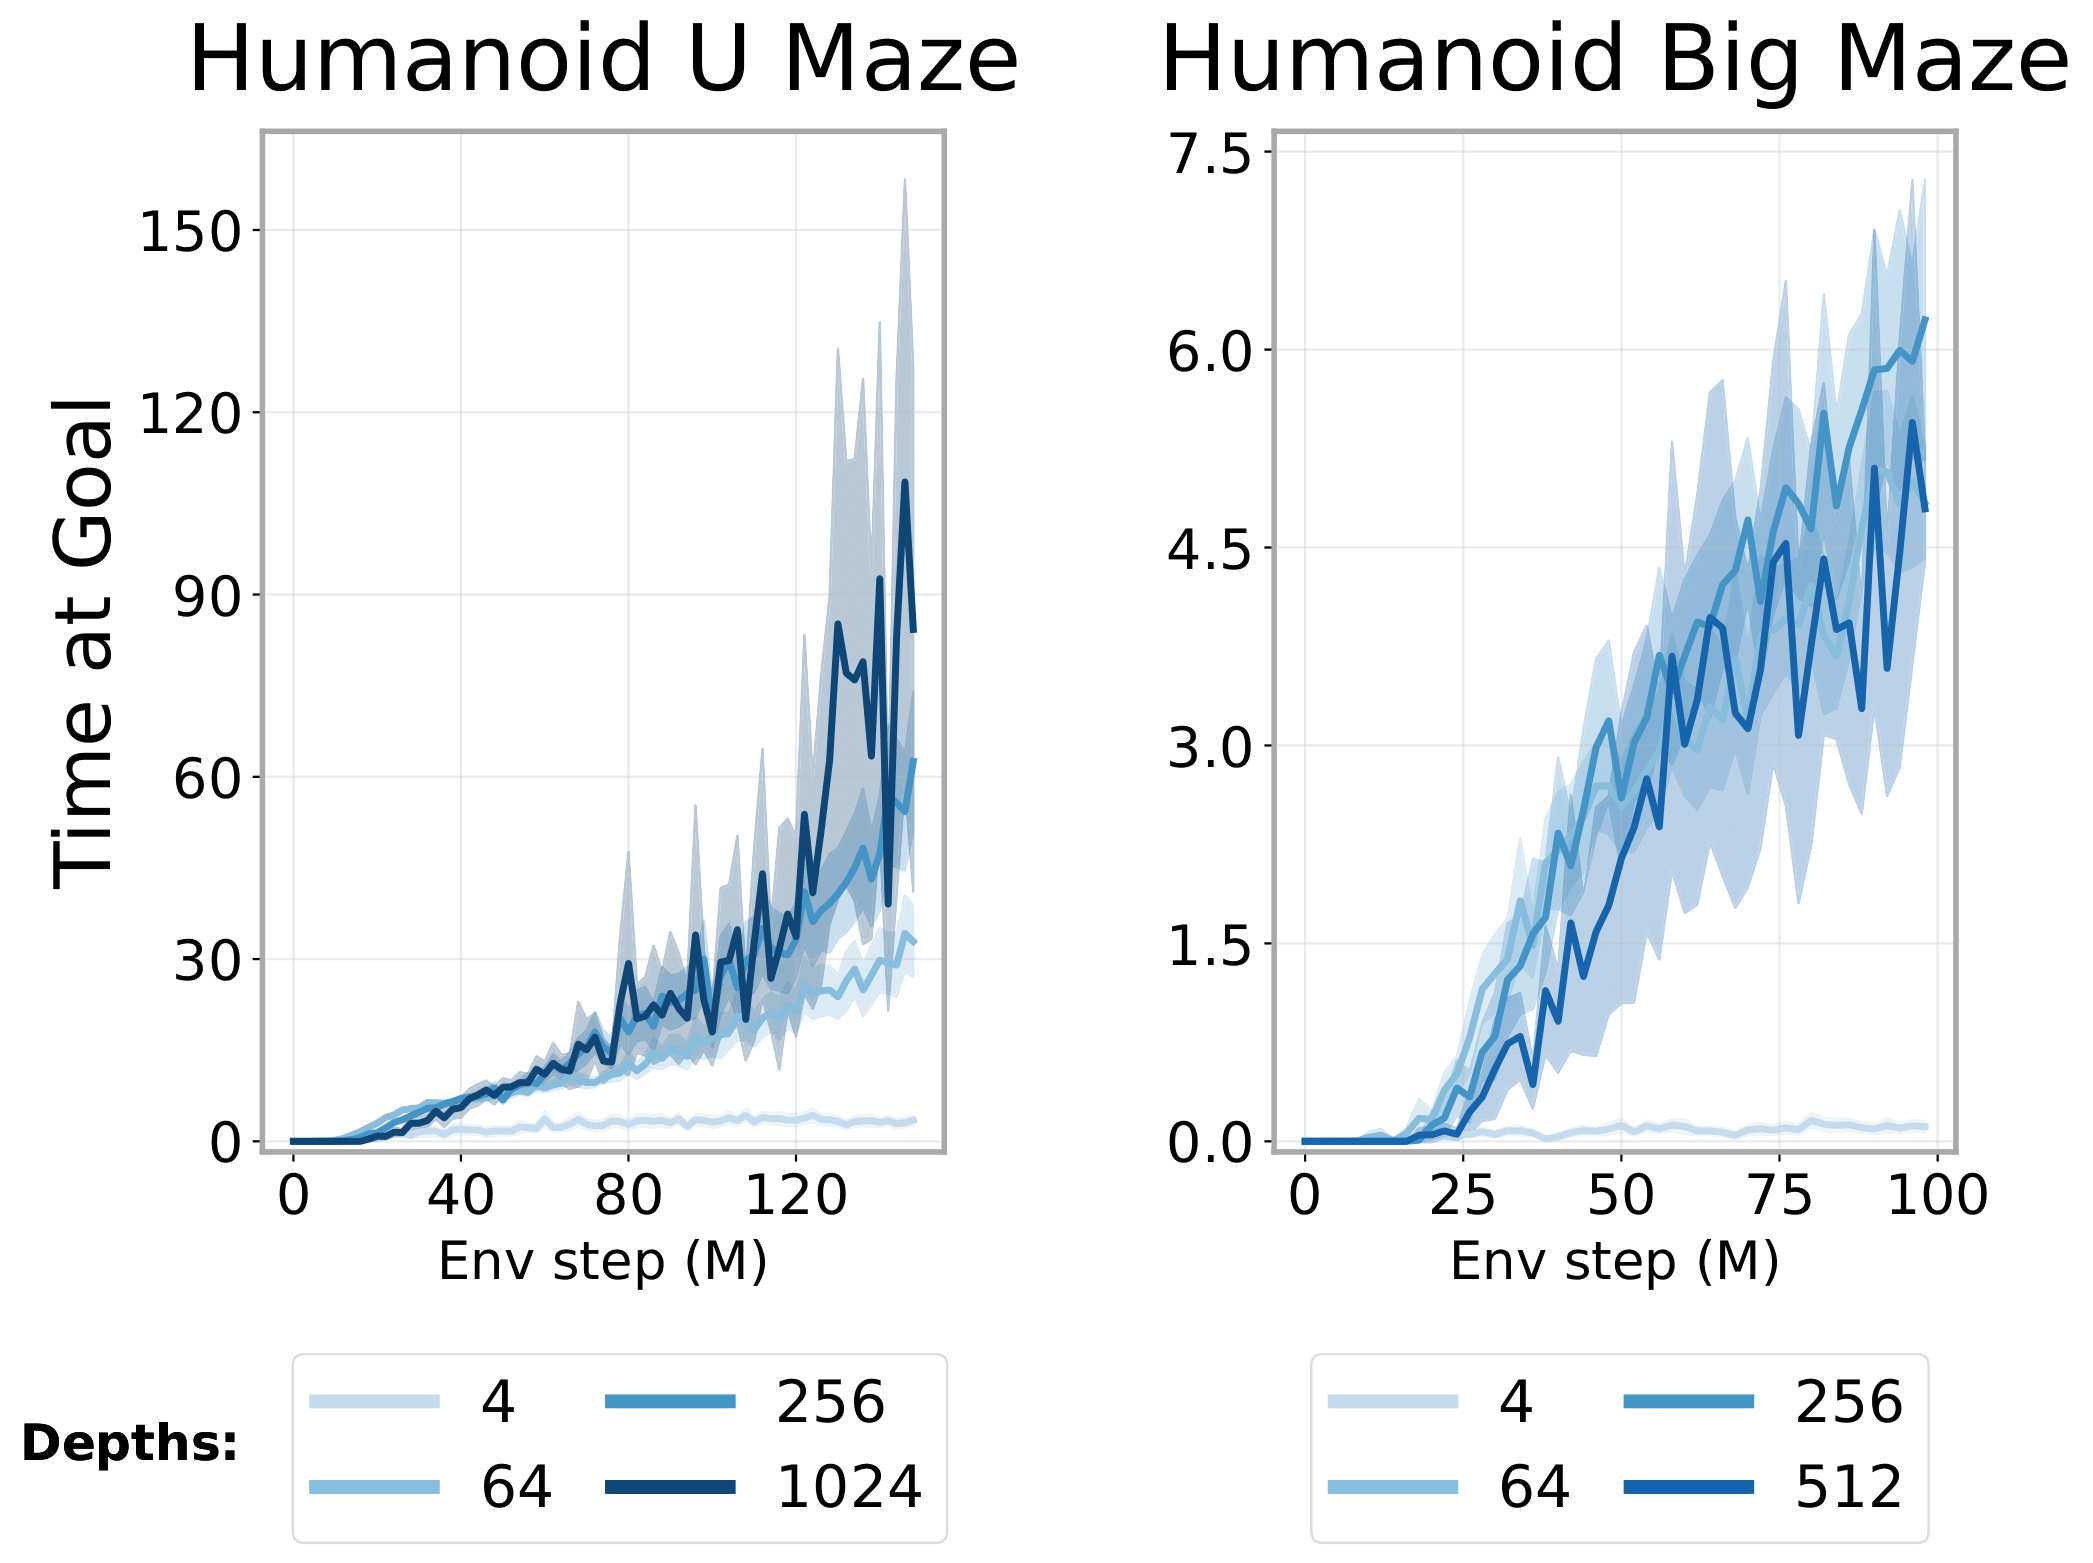
\includegraphics[width=\linewidth]{figures/depth_scaling_limits_2.png}
\caption{Time at goal versus environment steps on Humanoid U Maze (left) and Humanoid Big Maze (right) for policy networks at several depths (lighter to darker blue). Deeper models tend to reach higher time at goal; shaded bands show run-to-run variability. \emph{Reproduced from} \cite{wang2025thousand}.}
\label{fig:depth_scaling_rl}
\end{figure}

\section{Reasoning, diversity, and evaluation of language models}
This section covers the most ground, and deliberately so---the interplay between reasoning quality, output diversity, and evaluation methodology is, in our view, the central tension in current LLM research.

Start with diversity. Jiang \emph{et al.}\ show that many independently trained models converge toward strikingly similar outputs and failure modes under broad prompts \cite{jiang2025hivemind}. This is somewhat surprising given how different these models' training pipelines are, and it raises hard questions about behavioral diversity, dataset design, and what happens when homogeneity meets safety-critical deployments. Figure~\ref{fig:hivemind} makes the convergence visually stark: the distribution of final answer tokens across models and prompts reveals patterns that look far more uniform than one might expect.

On the architecture side, Qiu \emph{et al.}\ propose a gated attention mechanism that mitigates known failure modes like attention sinks while introducing useful non-linearity and sparsity into the attention map \cite{qiu2025gated}. The result is improved stability and long-context usability---a concrete engineering contribution that addresses a problem the Background section flagged.

Reasoning itself is being pushed in several directions at once. Song illustrates multi-scale CoT fusion for biological reasoning with large language models, where getting the \emph{structure} of the explanation right matters as much as the final answer \cite{song2026mscot}. Meanwhile, for smaller or parameter-efficient models, Sinha \emph{et al.}\ offer dynamic recursive CoT with meta-reasoning---a way to stretch reasoning capacity without proportionally growing the backbone \cite{sinha2025drcot}. Notably, this raises the question of whether recursive and multi-scale approaches will eventually converge into a unified framework, or whether they address fundamentally different bottlenecks.

What ties these threads together is a simple but underappreciated point: reasoning quality depends not just on architecture or training alone, but on how diversity and failure modes are measured. Better models and better evaluation must advance together.

\begin{figure}[!t]
  \centering
  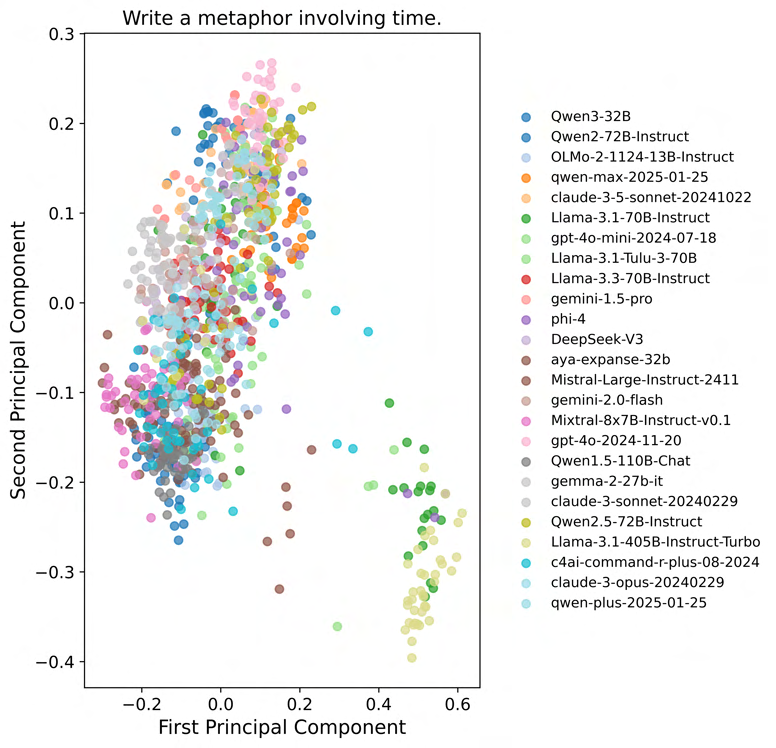
\includegraphics[width=\linewidth]{figures/hivemind.png}
  \caption{Distribution of final answer tokens across models and prompts. Each row is a model variant; columns are prompts and answer tokens are color-coded. Horizontal bars show the mean answer token distribution across all prompts; vertical bars show the model distribution across all prompts. \emph{Reproduced from} \cite{jiang2025hivemind}.}
  \label{fig:hivemind}
  \end{figure}

\section{Inference compute, theory, and memory efficiency}
Two problems, one hardware budget. Ellis-Mohr \emph{et al.}\ develop a theory of \emph{inference compute scaling}, casting test-time reasoning as search through a space of skills or procedures with a stochastic structure \cite{ellis2026inference}. The key insight is that extra compute at inference translates into measurable gains in problem-solving---but only when the search process is well aligned with the task. That ``only when'' matters. Independently, Staniszewski and {\L}a\'{n}cucki address the memory side: they propose transform coding for KV cache compression so that stored activations remain usable while shrinking their footprint \cite{staniszewski2026kv}.

These two efforts interact in an important way. Cheapening the KV cache enables longer or wider inference processes within the same hardware budget. In other words, scaling ``thinking time'' and scaling ``context memory'' are not independent levers---gains on one front relax constraints on the other. It is worth emphasizing that joint optimization of both remains largely unexplored, as we discuss further in Section~VIII.

\section{Failure modes in multi-agent LLM systems}
How can we evaluate the efficiency of an LLM agent system, and why do they fail? Cemri \emph{et al.}\ approach this question empirically: they evaluate seven MAS frameworks using over 1,600 human-annotated execution traces and construct MAST (Multi-Agent System Failure Taxonomy), a taxonomy of 14 failure modes grouped into three categories: system design and specification failures (FC1), inter-agent misalignment (FC2), and task verification problems (FC3) \cite{cemri2025multiagent}.

The resulting dataset, MAST-Data, serves as an empirical reference for an automatic annotation pipeline based on LLM-as-a-judge, which achieves 94\% agreement with human experts ($\kappa = 0.77$)---a figure below the human inter-annotator consensus ($\kappa = 0.88$), a gap the authors acknowledge but do not analyze in depth. This automation enables large-scale diagnosis without continuous manual validation.

What distinguishes this work from the single-agent evaluations discussed in Section~IV is that coordination across multiple agents introduces qualitatively distinct sources of error: broken communication between agents, redundant computation, and error propagation that no single-agent benchmark can detect. This connects directly to the homogeneity problem discussed earlier: if individual models converge in their outputs, shared blind spots do not cancel out in a MAS---they are amplified.

\section{Robotics and lightweight human feedback}
Biyik surveys how robots can be trained from natural, low-burden human feedback---preferences, rankings, language corrections, light interventions---rather than full teleoperation alone \cite{biyik2025robots}. The motivation is practical: non-expert users do not provide dense demonstrations, and real-time safety constraints rule out unconstrained autonomy.

This robotics perspective sharpens every theme we have discussed. Autonomy and reasoning must remain steerable. Lightweight supervision is often the only scalable alignment mechanism available in the field. And the gap between laboratory evaluation (as noted in Section~V) and messy real-world deployment is nowhere more apparent than in embodied agents interacting with people.

\section{Discussion}
The works surveyed here reveal several productive tensions, and we think it is worth being direct about what they imply.

Scaling depth and inference compute can produce qualitatively new capabilities \cite{wang2025thousand,ellis2026inference}. But as Jiang \emph{et al.}\ demonstrate, independently trained models converge toward homogeneous outputs \cite{jiang2025hivemind}. Raw scale, by itself, does not buy diversity or robustness. This tension is unresolved and, in our view, underappreciated.

Richer reasoning---whether through multi-scale CoT \cite{song2026mscot}, dynamic recursive CoT \cite{sinha2025drcot}, or gated attention \cite{qiu2025gated}---improves answer quality. The cost, however, is real: increased memory and compute demands that KV cache compression only partially offsets \cite{staniszewski2026kv}. As we noted in Section~VI, joint optimization of search depth and cache budget is still an open problem.

Moving to multi-agent systems amplifies both promise and peril. MAST documents 14 distinct failure modes that standard single-agent benchmarks cannot detect \cite{cemri2025multiagent}. And the robotics perspective reminds us that capable systems must remain steerable by non-expert users; lightweight feedback may be the only scalable alignment mechanism in real deployment \cite{biyik2025robots}.

Several concrete research gaps stand out. First, we need benchmarks that reward behavioral diversity, not just average accuracy---the homogeneity findings demand this. Second, failure taxonomies like MAST should be extended beyond the seven frameworks studied, and the LLM-as-a-Judge pipeline ($\kappa=0.88$) needs validation on out-of-distribution agent architectures. Third, joint optimization of inference-time search depth and KV cache budget remains essentially untouched. Finally, aligning increasingly autonomous multi-agent pipelines with human intent through lightweight feedback is largely unexplored territory that bridges the robotics and LLM communities.

One question we find genuinely unresolved: is the homogeneity observed across independently trained models a fundamental consequence of current training paradigms (large-scale pretraining on overlapping web data followed by RLHF), or can it be broken by architectural or data-level interventions without sacrificing quality? If the former, the implications for safety-critical deployment are serious and may require rethinking how we compose and deploy model ensembles.

\section{Conclusion}
This survey has examined ten recent works spanning five themes in deep learning: depth scaling in self-supervised reinforcement learning, reasoning and diversity in language models, inference-time compute theory and memory efficiency, failure modes in multi-agent LLM systems, and human-feedback-driven robot learning.

The core finding, stated plainly, is this: capability gains at one level---deeper networks, longer reasoning chains, wider agent pipelines---introduce new failure modes and resource constraints that do not resolve themselves with further scaling. They require dedicated study. Homogeneity across independently trained models, silent error propagation in multi-agent systems, and memory bottlenecks at inference are concrete examples.

These are just examples of the diverse methods that are being probed in the field to expand both the scale and efficiency of deep learning models. While a lot may prove to be dead ends or prove technically or economically infeasible, they still hold inherent value in steering the evolution of the field.

\section{Limitations}
A note about the survey's scope. It covers a curated and necessarily narrow slice of a vast, rapidly moving field. Each source cited connects to broader literatures we have not reviewed. Readers seeking deeper coverage of reinforcement learning theory should consult the model-based RL and world-models literature; for LLM alignment, the RLHF and constitutional AI lines of work extend the preference-learning thread; for multi-agent coordination, game-theoretic and mechanism-design perspectives complement the empirical failure taxonomy of MAST \cite{cemri2025multiagent}.

We close with what we see as the bottom line. Responsible deployment of advanced AI systems will require simultaneous progress on capability, reliability, efficiency, and human oversight. None of these is a solved problem, and it remains unclear whether progress on any single front can substitute for the others.

\section*{Acknowledgment}
The authors would like to especially thank Ph. D. José Antonio Cantoral Ceballos for his guidance and support during their initiation in the field of deep learning and artificial intelligence.

\begin{thebibliography}{00}

\bibitem{wang2025thousand}
K. Wang, I. Javali, M. Bortkiewicz, T. Trzci\'{n}ski, and B. Eysenbach, ``1000 Layer Networks for Self-Supervised RL: Scaling Depth Can Enable New Goal-Reaching Capabilities,'' 2026, arXiv:2503.14858. [Online]. Available: \url{https://arxiv.org/abs/2503.14858}

\bibitem{qiu2025gated}
Z. Qiu \emph{et al.}, ``Gated Attention for Large Language Models: Non-linearity, Sparsity, and Attention-Sink-Free,'' in \emph{Advances in Neural Information Processing Systems} (NeurIPS), 2025.

\bibitem{jiang2025hivemind}
L. Jiang \emph{et al.}, ``Artificial Hivemind: The Open-Ended Homogeneity of Language Models (and Beyond),'' in \emph{Advances in Neural Information Processing Systems} (NeurIPS), Datasets and Benchmarks Track, 2025.

\bibitem{sinha2025drcot}
A. Sinha, O. C. Umakanthan, and S. Gajendran, ``DR-CoT: Dynamic Recursive Chain of Thought With Meta Reasoning for Parameter Efficient Models,'' \emph{Sci. Rep.}, vol.~15, art.~34773, 2025, doi: 10.1038/s41598-025-18622-6.

\bibitem{ellis2026inference}
A. R. Ellis-Mohr, A. K. Nayak, and L. R. Varshney, ``A theory of inference compute scaling: Reasoning through directed stochastic skill search,'' \emph{Phil. Trans. R. Soc. A}, vol.~384, no.~20240510, 2026, doi: 10.1098/rsta.2024.0510.

\bibitem{staniszewski2026kv}
K. Staniszewski and A. {\L}a\'{n}cucki, ``KV Cache Transform Coding for Compact Storage in LLM Inference,'' 2026, arXiv:2511.01815. [Online]. Available: \url{https://arxiv.org/abs/2511.01815}

\bibitem{song2026mscot}
Z. Song, ``MS-CoT: Multi-scale chain-of-thought fusion for interpretable biological reasoning with large language models,'' \emph{Comput. Biol. Med.}, vol.~203, p.~111467, 2026, doi: 10.1016/j.compbiomed.2026.111467.

\bibitem{xu2025reasoning}
F. Xu, ``Toward large reasoning models: A survey of reinforced reasoning with large language models,'' \emph{Patterns}, vol.~6, no.~2, p.~101370, 2025, doi: 10.1016/j.patter.2025.101370.

\bibitem{biyik2025robots}
E. B{\i}y{\i}k, ``Training robots with natural and lightweight human feedback,'' \emph{AI Mag.}, 2025, doi: 10.1002/aaai.70037.

\bibitem{cemri2025multiagent}
M. Cemri, M. Z. Pan, S. Yang, L. A. Agrawal, B. Chopra, R. Tiwari, K. Keutzer, A. Parameswaran, D. Klein, K. Ramchandran, M. Zaharia, J. E. Gonzalez, and I. Stoica, ``Why Do Multi-Agent LLM Systems Fail?'' in \emph{Advances in Neural Information Processing Systems} (NeurIPS), Datasets and Benchmarks Track, 2025, arXiv:2503.13657. [Online]. Available: \url{https://arxiv.org/abs/2503.13657}

\end{thebibliography}

\end{document}